\documentclass{article}

\usepackage[final]{neurips_2018} % provided style file

\usepackage[utf8]{inputenc} % allow utf-8 input
\usepackage[T1]{fontenc}    % use 8-bit T1 fonts
\usepackage{hyperref}       % hyperlinks
\usepackage{url}            % simple URL typesetting
\usepackage{booktabs}       % professional-quality tables
\usepackage{amsfonts}       % blackboard math symbols
\usepackage{nicefrac}       % compact symbols for 1/2, etc.
\usepackage{microtype}      % microtypography

\usepackage{tabularx} % For tables with specified width
\usepackage{hyperref} % For hyperlinks
\usepackage{booktabs} % For better table lines
\usepackage{graphicx} % For including images
\usepackage{subcaption} % For subfigures

\bibliographystyle{plainnat}

\title{Predicting Cell Types in Non-Human Single Cell RNA Sequencing Data}

\author{
  Sean Connelly \\
  % examples of more authors
  \And
  Ryan Videgar-Laird \\
  \AND
  Stephanie Ting \\
}

\begin{document}

\maketitle

\section{Introduction}
\label{intro}

Single cell RNA sequencing data is eventually processed into a gene expression matrix, which has dimensions of m cells x n genes. After performing quality control steps, normalizing and scaling this gene expression matrix, this matrix undergoes dimensionality reduction to compress this dataset that contains many features (genes) to see how these cells relate to one another. The patterns of how cells vary compared to one another can be clustered using any algorithm of one’s choosing. The resulting clusters represent certain types of cells that need to be characterized and classified.

Classifying single cells has mainly focused on utilizing three categories of techniques. The first class of techniques annotate these clusters through comparing the differential expression (greater number of counts) of the genes in a given cluster with every other cluster through statistical tests, like the Wilcoxian rank sum test. These differentially abundant genes in each cluster can be compared to experimentally validated genes that characterize cell types to identify the label for that cluster. The second class of techniques correlates the newly generated dataset with a reference dataset to annotate cell clusters. This reference dataset can be other single cell RNA sequencing data or bulk RNA sequencing of specific cell types individually or over a time series. Lastly, the third class of techniques uses supervised learning, which utilizes previously generated data to train a model to classify cell types. Some examples of potential models to implement could be logistic regression, support vector machine or random forest, to name a few.

Many of these tasks have been focused on human data, where there has been much focus on diseases, like different forms of cancer, that affect many people domestically, but not much focus on diseases that have broad impacts globally. One such disease is malaria, a parasitic infection that resulted in 247 million cases in 2021 and causes a large burden of morbidity and mortality globally [world malaria report]. Malaria has a complex life cycle, which starts in the mosquito vector to result in infection of a human host. When individuals are sick with malaria, the parasite replicates in the blood cells and causes these blood cells to lyse when the parasite replicates. These replication stages have unique gene expression patterns and single cell RNA sequencing provides a key benefit to further understand how these genes change per cell stage. These same concepts can be applied to other neglected diseases and hosts. From looking at developmental trajectories in zebrafish [cite] to COVID-19 response in non-human primates [cite] to single cell RNA sequencing of other parasitic diseases [citations], we would like to build a powerful, simple and efficient model that can classify cell types on this source of data.



\subsection{Related Work}


\subsection{Methods}
\begin{itemize}

\item QC dataset to normalization
\item use processed gene expression matrix to perform one hot encoding as our embedding and learn with the one hot encoding and the processed gene exp matrix

\item implement the single head attention network

\item supervised

  \begin{itemize}
    \item input: normalized gene expression matrix and the one hot encoding
    \item single head attention
    \item output: classification of cell type
  \end{itemize}
  
  \item unsupervised
    \begin{itemize}
      \item input: normalized gene expression matrix and the one hot encoding
      \item single head attention
      \item output: embedding for each gene for each cell
      \item weights: what are updated during your loss function, can pull and look at them
    \end{itemize}

\end{itemize}

\section{Preliminary Results}

\begin{table}[h]
  \caption{Summary of datasets that will be used in this study.}
  \label{tab:summary}
  \centering
  \begin{tabularx}{\textwidth}{lXll}
    \toprule
    \textbf{Host} & \textbf{Source} & \textbf{Reference} & \textbf{Cells} \\
    \midrule
    Parasite & \href{https://github.com/vhowick/MalariaCellAtlas/tree/master/Expression_Matrices10X/pf10xIDC}{GitHub} & Howick et al. 2019 & 6,737 \\
    \midrule
    Parasite & GSE146737 & Wendt et al. 2020 & 43,642 \\
    \midrule
    Parasite & \href{https://zenodo.org/record/5163554\#.YQvu2ZNKjUo}{Zenodo} & Briggs et al. 2021 & 8,599 \\
    \midrule
    Parasite & \href{https://github.com/umbibio/scBabesiaAtlases}{GitHub} & Rezvani et al. 2022 & 8,719-12,910 \\
    \midrule
    Human & TENxPBMCData R package (Kasper et al. 2021) & 10X Genomics & 3,000 \\
    \midrule
    Human & scRNAseq package (Risso and Cole, 2021) & Lawlor et al. 2017 & 978 \\
    \midrule
    Human & GSE151530 & Ma et al. 2021 and Ma et al. 2022 & 56,721 \\
    \midrule
    Mouse & scRNAseq package (Risso and Cole, 2021) & Zeisel et al. 2015 & 3,005 \\
    \midrule
    Zebrafish & GSE106587 & Farrell et al. 2018 & 38,731 \\
    \midrule
    Non-human primate & GSE156755 & Speranza et al. 2021 & 100,795 \\
    \bottomrule
  \end{tabularx}
\end{table}

\begin{figure}
  \centering
  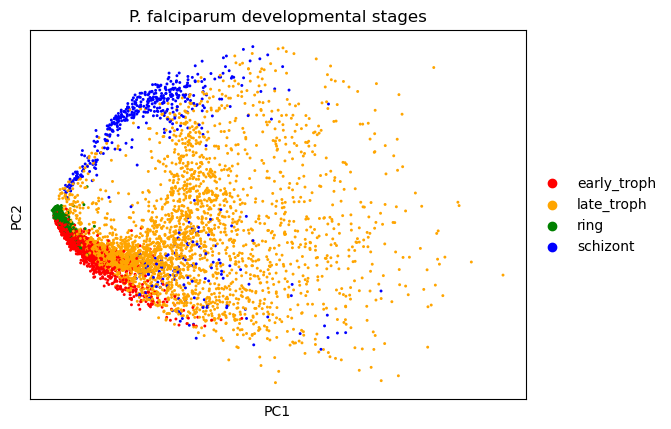
\includegraphics[width=0.8\textwidth]{figures/pca_Pf.png}
  \caption{Principal components analysis of \textit{P. falciparum} single cell RNA sequencing data, colored by lifecycle stage.}
\end{figure}

\begin{figure}[htbp]
  \centering
  
  \begin{subfigure}[b]{0.3\textwidth}
      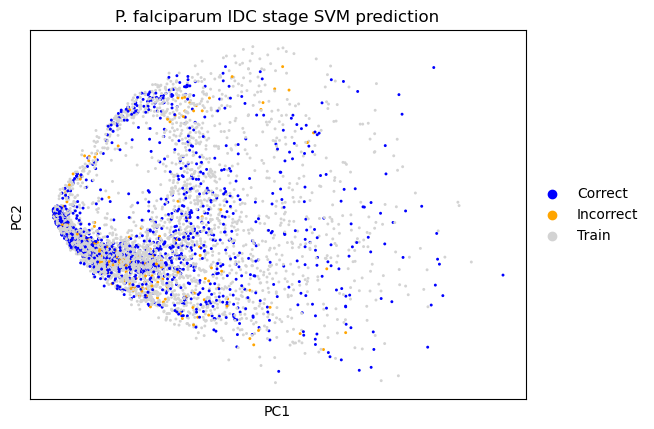
\includegraphics[width=\textwidth]{figures/pca_Pf_prediction_SVM.png}
      \caption{PCA of predictions from SVM model.}
      \label{fig:sub1}
  \end{subfigure}
  \hfill
  \begin{subfigure}[b]{0.3\textwidth}
      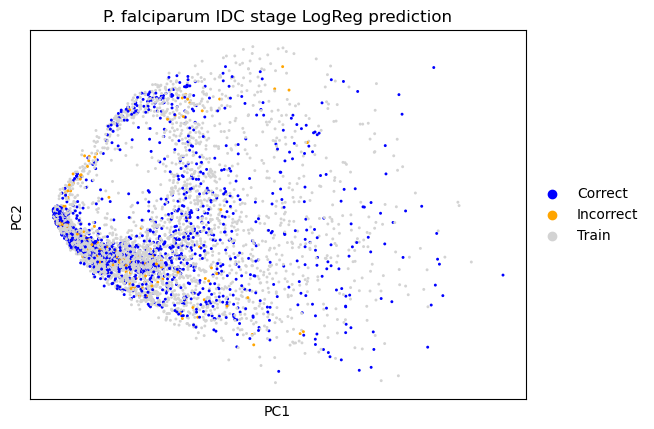
\includegraphics[width=\textwidth]{figures/pca_Pf_prediction_LogReg.png}
      \caption{PCA of predictions from logistic regression model.}
      \label{fig:sub2}
  \end{subfigure}
  \hfill
  \begin{subfigure}[b]{0.3\textwidth}
      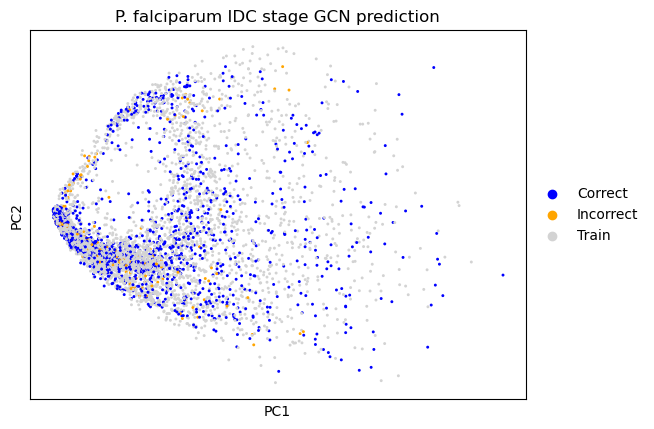
\includegraphics[width=\textwidth]{figures/pca_Pf_prediction_GCN.png}
      \caption{PCA of predictions from graph convolutional network model.}
      \label{fig:sub3}
  \end{subfigure}
  
  \caption{Model performance visualized on PCA plots.}
  \label{fig:main}
\end{figure}

\begin{figure}
  \centering
  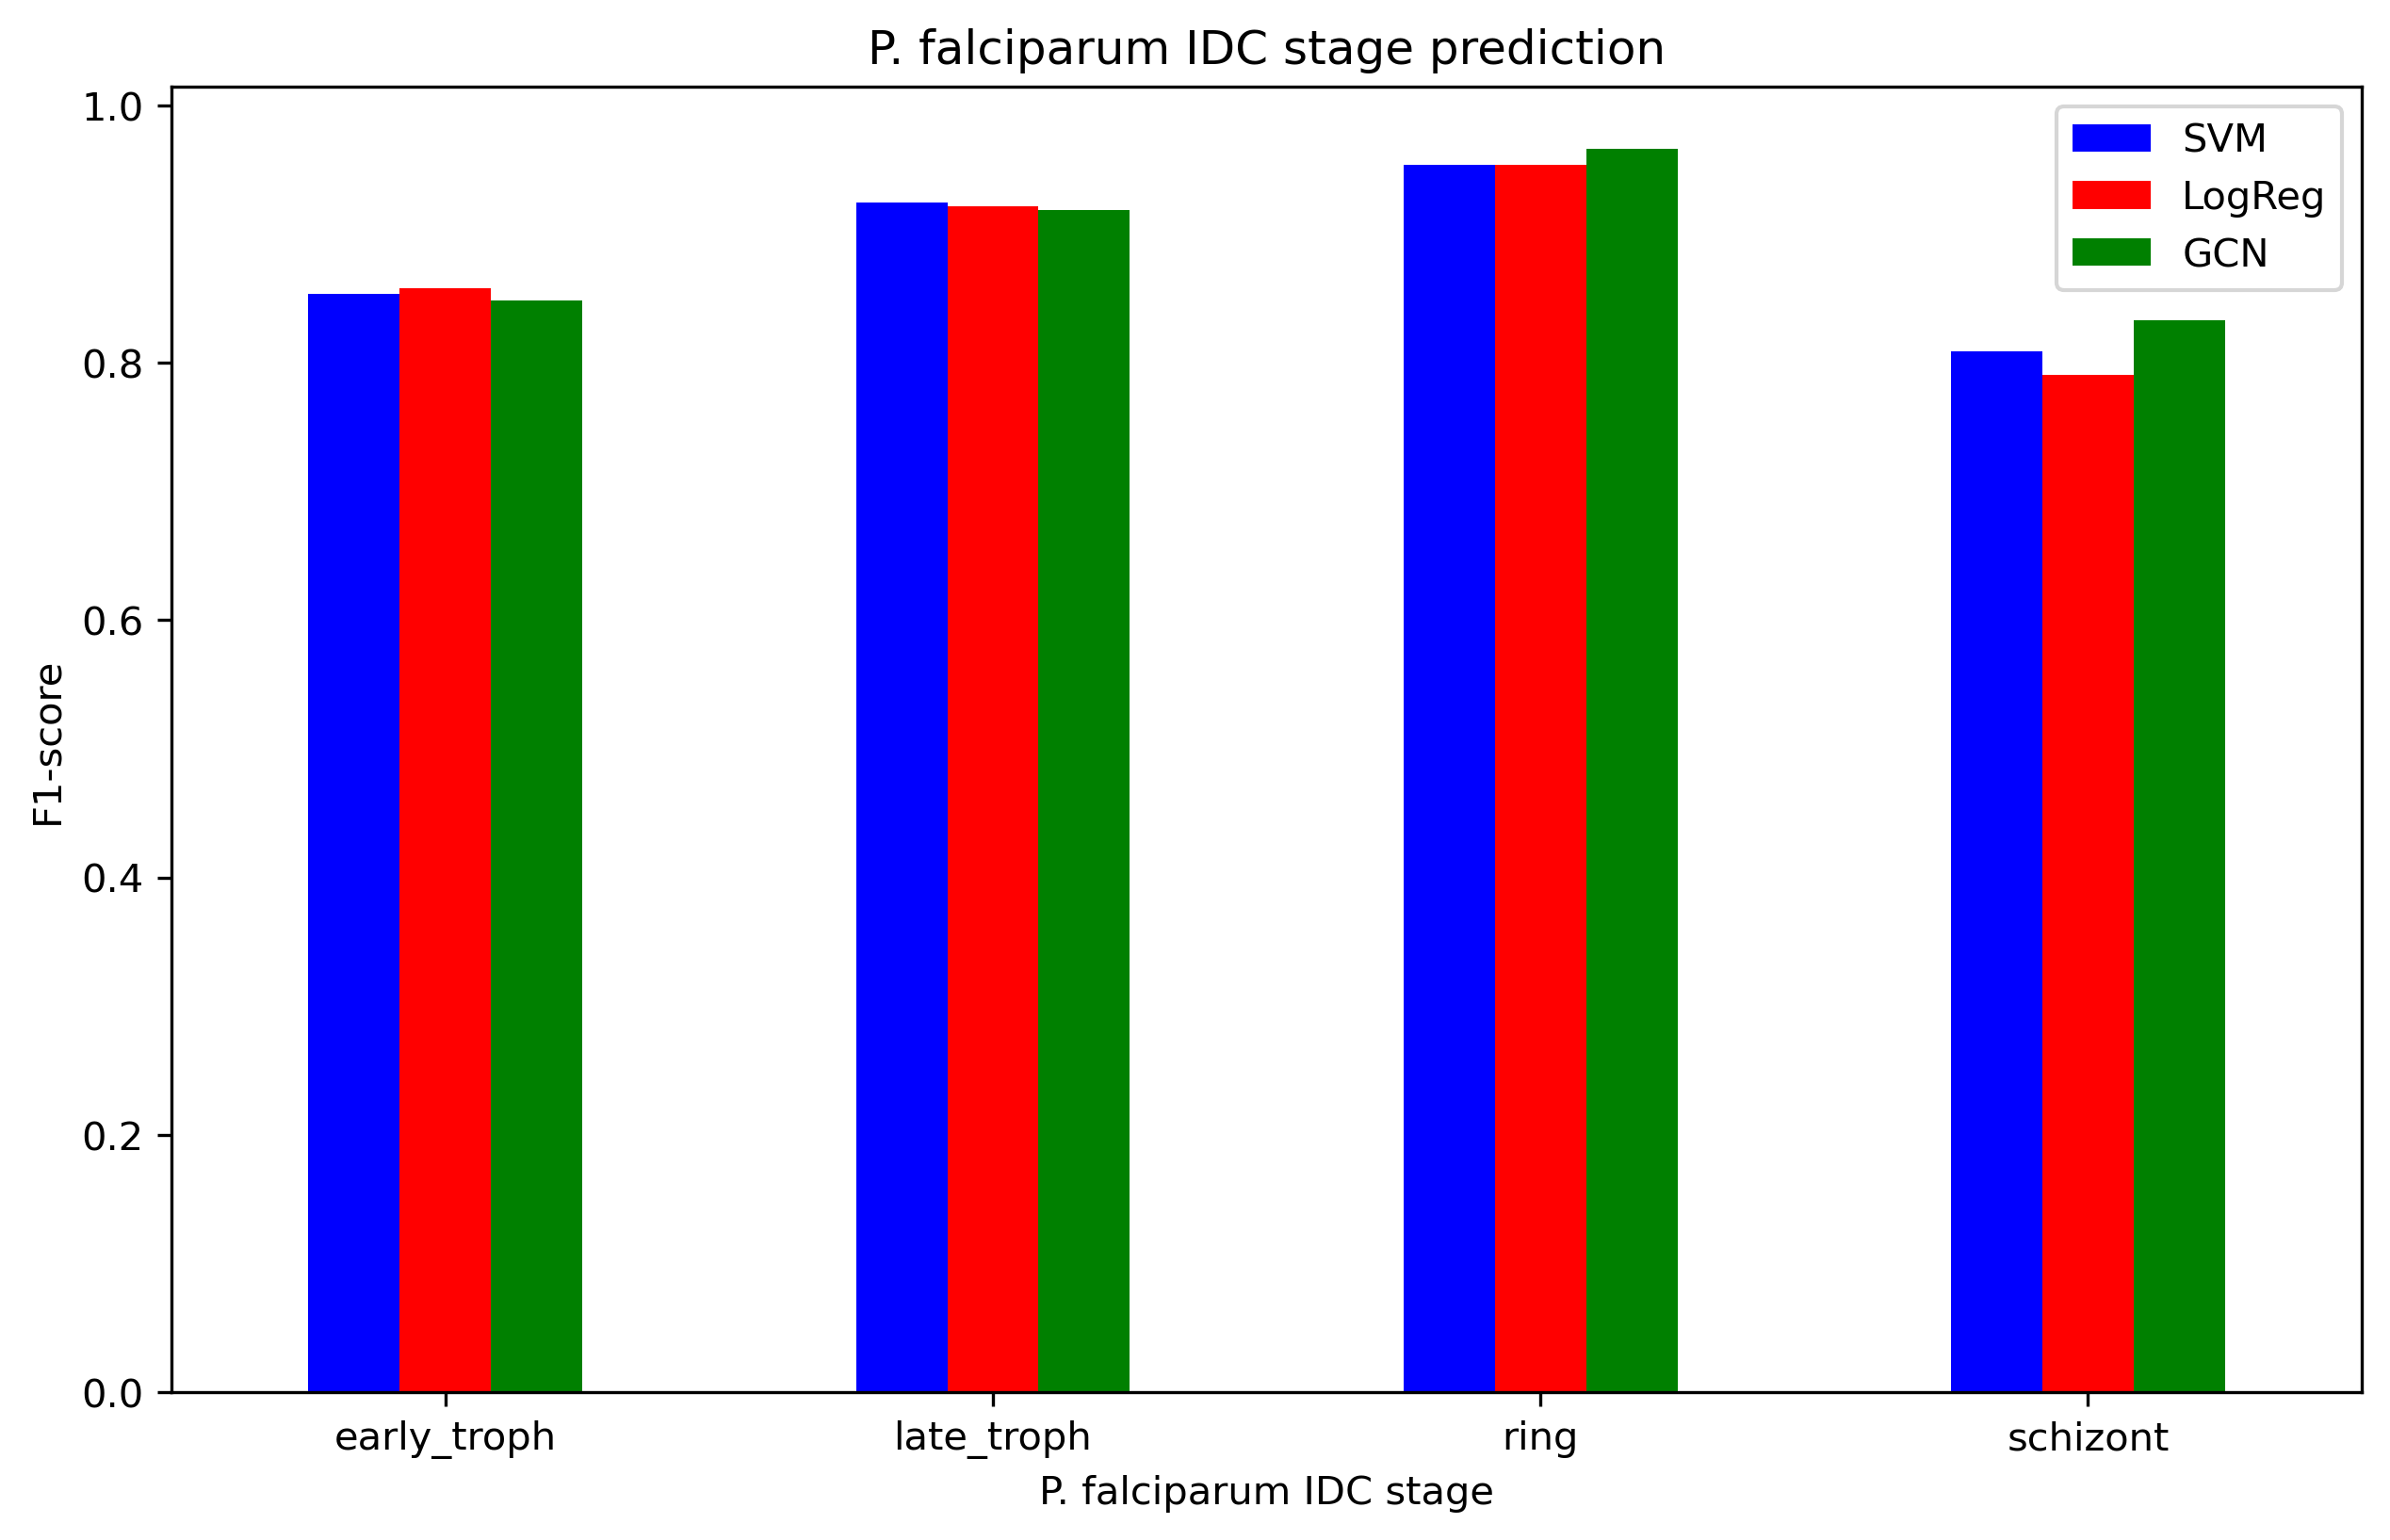
\includegraphics[width=0.8\textwidth]{figures/Pf_prediction.png}
  \caption{Prediction accuracy of models on \textit{P. falciparum} single cell RNA sequencing data.}
\end{figure}


\cite{yangScBERTLargescalePretrained2022}

\bibliography{midway_report}

\end{document}

